\documentclass[editmode]{EPFL_BEAMER}
% To change the slides size go to EESD.cls file and edit the preamble as explained.

% ---- Add your Meta-data to the PDF (Copyrights Kinda!) ----
\hypersetup{
  pdfinfo={
    Title={Presentation: 3D finite element modeling of historical masonry walls},
    Author={Mahmoud S. Shaqfa, Katrin Beyer},
    Subject={EPFL - ENAC - EESD Lab},
    Keywords={Stone masonry, Detailed micro-mechanical, 3D micro-structure}
  }
}

% Important packages to be called
\usepackage{subcaption} % for adding sub-figures
\usepackage{graphicx}
\usepackage{tikz} % for cool graphics and drawings
\usepackage{dirtytalk}
\usepackage[absolute,overlay]{textpos} % To place the figures by coordinates (x,y) - Beamer doesn't support floats XD

% \usepackage[absolute,overlay, showboxes]{textpos} % To place the figures by coordinates (x,y) - Beamer doesn't support floats XD

% To define a grid that helps in positioning






\usepackage{multicol} % To adjust items and stuff automatically in a number of a pre-specified columns
\graphicspath{{Figures/}}
\usepackage[utf8]{inputenc}
\usepackage{amsmath}
\usepackage{amsfonts}
\usepackage{amssymb}
\usepackage{lipsum} % Just a dummy text generator
\usepackage{hyperref}
% fonts packages
\usepackage{ragged2e} % Justified typesetting


% For References Only
% \usepackage[style=authortitle,backend=bibtex]{biblatex}
\usepackage[style=authoryear, natbib=true, backend=biber, maxbibnames=9, maxcitenames=2, uniquelist=false]{biblatex}

\addbibresource{References.bib} % Call the references database
\AtBeginBibliography{\tiny} % Specify font size (Size matters)
\renewcommand{\footnotesize}{\tiny}

% For adding code blocks
\usepackage{listings}
\lstset
{
    language=[LaTeX]TeX,
    breaklines=true,
    basicstyle=\tt\scriptsize,
    keywordstyle=\color{blue},
    identifierstyle=\color{magenta},
    commentstyle=\color{red},
    rulecolor=\color{black},
    numbers=left,
    numberstyle=\tiny\color{black},
    % framexleftmargin=15pt,
    frame = single,
}

\author{~\vspace{5mm} Mahmoud S. Shaqfa}
% \author{Mahmoud S. Shaqfa \newline~\newline Prof. Katrin Beyer}
\title[Stone masonry micromodeling]{A virtual microstructure generator for 3D stone masonry walls}
\supervisor{Katrin Beyer}

\institute[ENAC]{\newline{\'Ecole Polytechnique F\'ed\'erale de Lausanne (EPFL)}{\vspace{2mm}\newline School of Architecture, Civil and Environmental Engineering (ENAC)}}
\subject{Candidacy Exam}
\date{May 2022}

\begin{document}

{ % <-- don't forget the scope resolution (Brackets) to limit the background change only for the cover page; otherwise, it will override the whole document's background :)
\usebackgroundtemplate{} % To add a background for this slide XD - Empty one
\coverpage{
\titlepage{~}
% To add additional text to the title components 
{\newline Supervisor: Prof. Katrin Beyer}
}
} % <-- and yeah close them too :)

% To define the cover-page here .. I prefer this
{
\usebackgroundtemplate{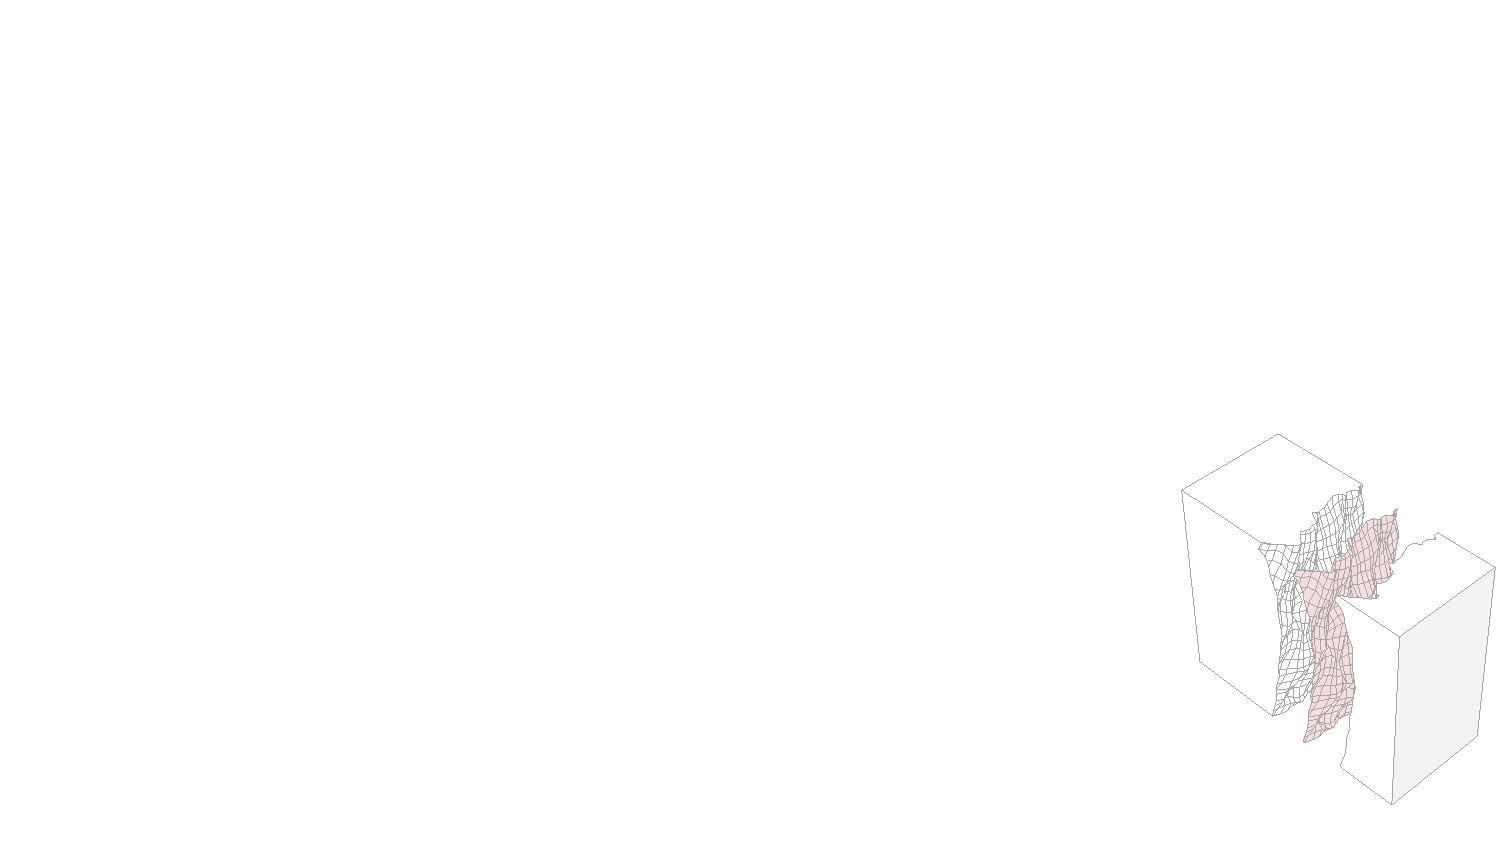
\includegraphics[width=1.\paperwidth, height=1.\paperheight]{cover169.pdf}} % To add a background for this slide XD - change it
\coverpage{
\titlepage{~}
% To add additional text to the title components 
{\newline Supervisor: Prof. Katrin Beyer}
}
}
{

{
\usebackgroundtemplate{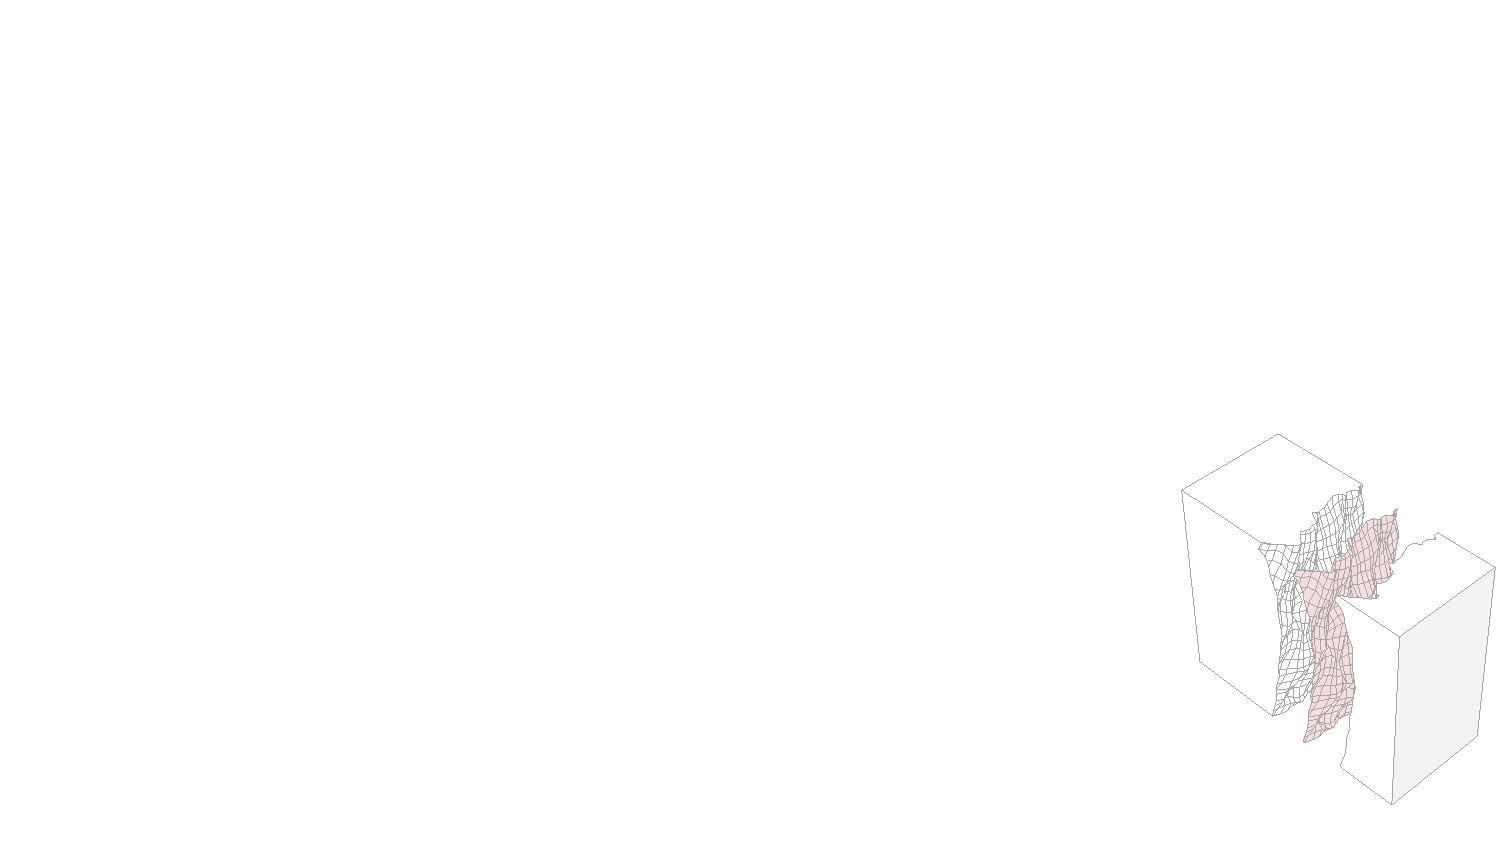
\includegraphics[width=1.\paperwidth, height=1.\paperheight]{cover169.pdf}} % To add a background for this slide XD - change it
\coverpageEPFL{
\titlepage{~}
}
}

% Add background and adjust the opacity
\usebackgroundtemplate{
\begin{tikzpicture}%
\node[opacity=0.1]{
\includegraphics[width=1.\paperwidth, height=1.\paperheight]{homer-simpson.jpg}
};%
\end{tikzpicture}
} % To add a background for this slide XD - Homer Simpson - Source: https://www.kcbi.org/to-be-understand-the-bible-we-need-to-listen-to-homer-simpson/

% \coverpage{
% \titlepage{~}
% % To add additional text to the title components 
% {\newline Supervisor: Prof. Katrin Beyer}
% }
}

\setbeamertemplate{logo}{} % To override the logo from the other slides and delete it completely


% -----------------------Table of contents TOC Three Styles
% Explicitly split the TOC if it's too long
% \begin{frame}[allowframebreaks]{Outlines}
% \tableofcontents[sections={1-3}] % Explicitly split TOC
% \framebreak
% \tableofcontents[sections={4-7}] % Explicitly split TOC
% \end{frame}

% % Just a normal TOC 
% \begin{frame}[allowframebreaks]{Outlines}
% \tableofcontents
% \end{frame}

% Use smart division for the TOC
\begin{frame}{Outlines}
\begin{multicols}{2}
\tableofcontents
\end{multicols}
\end{frame}

% -----------------------Introduction
\section{Introduction}

\breakingframe{
% \begin{textblock*}{3cm}[0.5,0.5](0.5\textwidth,  0.5\textheight)
% \Huge\textbf{\textcolor{black}{Introduction}}
% \end{textblock*}
}

\blackbreakingframe{
% \begin{textblock*}{3cm}[0.5,0.5](0.5\textwidth,  0.5\textheight)
% \Huge\textbf{\textcolor{black}{Introduction}}
% \end{textblock*}
}

\blackbreakingframe{
\begin{textblock*}{3cm}[0.5,0.5](0.55\textwidth,  0.5\textheight)
    \Huge\textbf{\textcolor{black}{Miss}\textcolor{white}{ion}}
\end{textblock*}
}

\cyanbreakingframe{
% \begin{textblock*}{3cm}[0.5,0.5](0.5\textwidth,  0.5\textheight)
% \Huge\textbf{\textcolor{black}{Introduction}}
% \end{textblock*}
}

\subsection{Copyright}
\begin{frame}[t]{Copyright}
\begin{textblock*}{13cm}(1.5cm,  2.0cm)
    {\fontfamily{qcr}\selectfont
    This file is a customized "beamer" template made for the EESD laboratory at EPFL (see \href{https://www.epfl.ch/labs/eesd/}{https://www.epfl.ch/labs/eesd/}). The author of this file is \textbf{Mahmoud S. Shaqfa}. This file is free: you can redistribute it and/or modify it under the terms of the GNU General Public License as published by    the Free Software Foundation, either version 3 of the License, or (at your option) any later version. This file is distributed in the hope that it will be useful, but WITHOUT ANY WARRANTY; without even the implied warranty of MERCHANTABILITY or FITNESS FOR A PARTICULAR PURPOSE.  See the GNU General Public License for more details. To receive a copy of GNU License refer to: \href{https://www.gnu.org/licenses/}{https://www.gnu.org/licenses/}
    }
\end{textblock*}
\end{frame}

\subsection{Cover page}
\begin{frame}[fragile]
\frametitle{Cover page}
    To define the cover page use the following code:
    \vspace{10pt}
    \begin{lstlisting}
    { % <-- Important to add those brackets; to affect only the background in this frame.
    \usebackgroundtemplate{\includegraphics[]{}} % <-- Define the background here
        \coverpage{
            \titlepage % make the title here
            {\newline Additional text like the supervisors, jury .. etc}
        }
        }
    } % <-- end of the environment
    \end{lstlisting}
    \vspace{10pt}
\end{frame}

\section{EESD logo}


\begin{frame}{Call another section}
    \lipsum[5]
\end{frame}

\begin{frame}{A citation example}
    In text citation example: \cite{SHAQFA2022} or \citep{SHAQFA2022}
    \newline~\newline
    Full citation entry: \fullcite{SHAQFA2022}
    \newline~\newline
    This is a footnote citation \footcite{SHAQFA2022}.
\end{frame}

\section{Comics}
\subsection{A nerdy one}
\begin{frame}{A comic}
    \begin{textblock*}{13cm}(2.0cm, 2.5cm)
        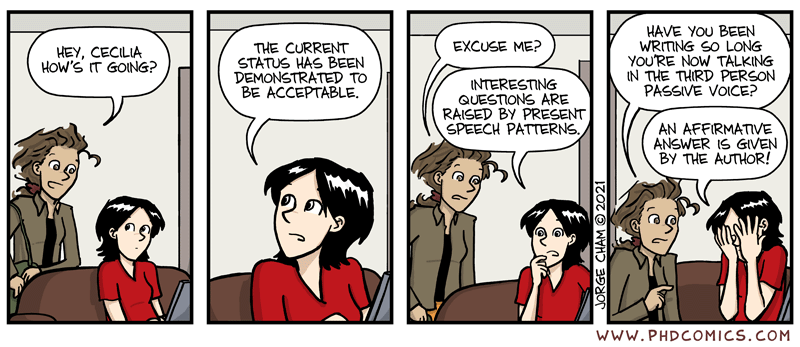
\includegraphics[width=1.0\textwidth]{phd102221s.png}
    \end{textblock*}
\end{frame}


\subsection{Horrible ones}
\begin{frame}{Another comic}
    \begin{textblock*}{13cm}(2.0cm, 2.5cm)
        
\includegraphics[width=1.0\textwidth]{phd102221.png}
    \end{textblock*}
\end{frame}

\begin{frame}{Ok the last one \dots}
    \begin{textblock*}{13cm}(2.0cm, 2.5cm)
        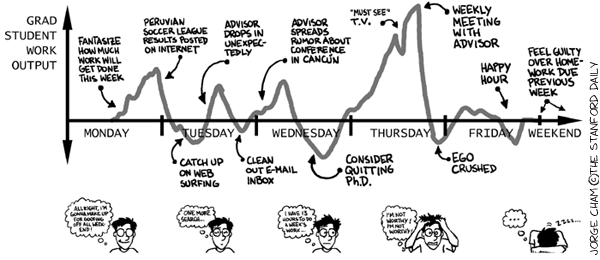
\includegraphics[width=1.0\textwidth]{phd050399s.png}
    \end{textblock*}
\end{frame}


% -----------------------References
% Thank you slide should be here
\breakingframe{
\begin{textblock*}{10cm}(3.2cm,4cm)
\Huge\textbf{\textcolor{black}{Merci de vo}\textcolor{white}{tre attention}}
\end{textblock*}
}

\cyanbreakingframe{
\begin{textblock*}{10cm}(3.2cm,4cm)
\Huge\textbf{\textcolor{black}{Merci de vo}\textcolor{white}{tre attention}}
\end{textblock*}
}

\blackbreakingframe{
\begin{textblock*}{10cm}(3.2cm,4cm)
\Huge\textbf{\textcolor{black}{Merci de vo}\textcolor{white}{tre attention}}
\end{textblock*}
}

% -----------------------References
{
\setbeamertemplate{bibliography item}{} % To fix the biblatex labelling issue with author-year style
\section{Bibliography}
% \begin{frame}[allowframebreaks]{\\References}\vspace{4pt}
\begin{frame}{References}\vspace{4pt}
\tiny{\printbibliography}
\end{frame}
\normalsize
}
\end{document}